\documentclass[11pt,a4paper]{article}
\usepackage[text={6.5in,10in},centering,a4paper]{geometry}
\usepackage{indentfirst}
\usepackage{setspace}
\usepackage{amssymb,amsmath} % Equations
\usepackage{tabularx} % Tables
\usepackage{graphicx,color} % Graphics, Figures
\usepackage[tight,footnotesize]{subfigure}
\usepackage{pgfgantt} % for gantt chart
\usepackage[hidelinks]{hyperref}
\usepackage[titletoc]{appendix}
\usepackage[nottoc,numbib]{tocbibind}
\usepackage[numbers]{natbib}
\usepackage[no-math]{fontspec}
\usepackage{xunicode} % for Thai fonts
\usepackage{xltxtra} % for Thai fonts

\def\figurename{รูปที่}
\def\tablename{ตารางที่}
\def\refname{เอกสารอ้างอิง}
\def\chaptername{บทที่}
\def\abstractname{\large Abstract}
\def\contentsname{สารบัญ}
\def\listfigurename{สารบัญรูป}
\def\listtablename{สารบัญตาราง}
\def\figurename{รูป}
\def\tablename{ตาราง}
\def\appendixname{ภาคผนวก}

\graphicspath{{figures/}} % create a director 'figures' in your local dir and all pics are kept here

%========== Thai Font ===========================
\XeTeXlinebreaklocale "th_TH"
\defaultfontfeatures{Scale=1.0, Mapping=tex-text} 
\setmainfont[Scale=1.2]{TH Sarabun New}
%========== Thai Font ===========================

\begin{document}
\thispagestyle{empty}
\begin{center}
    \doublespacing
    {\LARGE \bf ข้อเสนอโครงงานวิศวกรรมไฟฟ้า วิชา 2102490}
    \vfill
    {
        \LARGE \bf
        % ชื่อโครงงานภาษาไทย
        อิเล็กทรอนิกส์กำลังสำหรับระบบเก็บเกี่ยวพลังงานชนิดเครื่องจักรกลไฟฟ้า \\[2ex]
        % ชื่อโครงงานภาษาอังกฤษ
        Power Electronics for Electromechanical Energy-Harvesting System
    }
    \vfill
    {\LARGE \bf นายณัฐพล กาบแก้ว เลขประจำตัว 6130176521}\\[2ex]
    {\LARGE \bf อาจารย์ที่ปรึกษา รศ.ดร. สุรพงศ์ สุวรรณกวิน}
    \vfill
    {\LARGE \bf ภาควิชาวิศวกรรมไฟฟ้า คณะวิศวกรรมศาสตร์}\\[2ex]
    {\LARGE \bf จุฬาลงกรณ์มหาวิทยาลัย}\\[2ex]
    {\LARGE \bf ปีการศึกษา 2564}
\end{center}

\newpage
\thispagestyle{empty}
\tableofcontents

\newpage
\setcounter{page}{1}
\section{บทนำ}
\subsection{ที่มาและความสำคัญของโครงงาน}
หัวข้อนี้เป็นการกล่าวถึง ความเป็นมา เหตุผล หรือแรงจูงใจ ที่ทำให้นิสิตเลือกหัวข้อโครงงานนี้ และประโยชน์หรือความสำคัญของโครงงานนี้ต่อการพัฒนาองค์ความรู้ในด้านต่างๆ เช่น ในเชิงวิชาการ เชิงเศรษฐกิจ เชิงวิศวกรรม ไม่ใช่กล่าวถึงการพัฒนาตัวนิสิตหรือสิ่งที่นิสิตจะได้รับ นิสิตอาจนำเสนอข้อมูล เช่น สถิติ ตาราง กราฟ เป็นต้น เพื่อสนับสนุนเหตุผล และความสำคัญ นิสิตควรเขียนแยกแต่ละประเด็นเป็นย่อหน้า การเขียนต้องกระชับ เข้าประเด็นโดยไม่อ้อมค้อม ซึ่งรวมถึงทุกส่วนในรายงานนี้ด้วย ไม่ควรอธิบายสิ่งที่เยิ่นเย้อและเป็นสิ่งที่รู้กันอยู่แล้ว เช่น “การประหยัดพลังงานเป็นสิ่งสำคัญที่ทุกคนต้องคำนึงถึง” “ในอนาคตหุ่นยนต์จะมีบทบาทเข้ามาทำงานแทนมนุษย์อย่างสิ้นเชิง” หรือ “ในยุคดิจิตอลจะช่วยให้มนุษย์สื่อสารและทำงานได้มีประสิทธิภาพมากขึ้นหากมีโครงข่ายสื่อสารทั่วโลก”


ในส่วนถัดมาให้อธิบายว่าหัวข้อโครงงานที่เลือกทำนี้ มีประเด็นปัญหาสำคัญอะไรบ้าง มีรายละเอียดหรือลักษณะของปัญหาอย่างไร มีใครที่เคยแก้ปัญหาลักษณะนี้หรือคล้ายกันมาก่อนบ้าง ถ้าโครงงานนี้เป็นการต่อยอด หรือปรับปรุงผลงานจากโครงงานที่ทำมาก่อนหน้า หรือจากวรรณกรรม ควรต้องชี้ว่าผลงานเก่ามีจุดด้อย หรือจุดอ่อนอะไร และโครงงานนี้จะช่วยแก้ไข หรือปรับปรุงอะไร ในการกล่าวถึงงานที่ผู้อื่นได้ทำมาแล้ว จะต้องใส่เอกสารอ้างอิงให้ชัดเจน เช่น บทความที่กล่าวถึงเรื่อง XX พบได้ใน ~\cite{WaJ:08} การคัดลอกผลงานของผู้อื่น ไม่ว่าทั้งหมดหรือบางส่วน โดยไม่อ้างอิงแหล่งที่มา ถือเป็นการกระทำที่ผิดต่อศีลธรรมและจรรยาบรรณ หากพบว่านิสิตมีการกระทำดังกล่าว นิสิตจะได้รับเกรด U หรือ F


ย่อหน้าสุดท้าย ให้อธิบายถึงสิ่งที่คาดหวังว่าจะได้เมื่อจบโครงงาน (ไม่ใช่สิ่งที่ตัวนิสิตจะได้รับ) และวิธีการที่ใช้ หรือแนวทางการดำเนินการของโครงงานนี้โดยย่อ พร้อมแสดงถึงข้อดี หรือประเด็นที่นำเสนอใหม่ในโครงงานนี้ หากมีแผนผังความคิด (Mind Map) ที่จะช่วยให้เข้าใจโครงสร้างของโครงงานได้โดยง่าย ก็ขอให้ใส่ในหัวข้อนี้ด้วย ความยาวรวมของหัวข้อนี้ไม่ควรยาวเกินสองหน้า

\subsection{วัตถุประสงค์ของโครงงาน}
วัตถุประสงค์ คือผลลัพธ์สุดท้าย (Outcome) ของโครงงาน วัตถุประสงค์จะคล้ายกับหัวข้อโครงงาน เพียงแต่มีรายละเอียดและความชัดเจนมากกว่าหัวข้อ วัตถุประสงค์ควรเล็งถึงสิ่งที่เป็นรูปธรรม เช่น ออกแบบและสร้างอุปกรณ์ (Device) ประดิษฐ์หรือหาระเบียบวิธี (Algorithm) หาพารามิเตอร์หรือสภาวะที่เหมาะสม (Characterization or Optimization) ออกแบบและสร้างระบบ (System Integration) ศึกษาและเปรียบเทียบ (Study and Comparison) พัฒนาซอฟต์แวร์ (Software Development) วัตถุประสงค์ไม่ควรเป็นเพียงการกระทำ (Actions) ของนิสิต เช่น เรียนรู้การใช้โปรแกรม MATLAB/Simulink ศึกษาการใช้งานไมโครโปรเซสเซอร์ ทำความเข้าใจคณิตศาสตร์ เรียนรู้การใช้งานและทดสอบเครื่องมือ เป็นต้น นิสิตควรเขียนวัตถุประสงค์ให้กระชับ ไม่ควรยาวเกินหกบรรทัด และสามารถแยกเป็นข้อๆ เพื่อความชัดเจนได้ (ไม่ควรเกินสามข้อ) เช่น
\begin{enumerate}
    \item เพื่อพัฒนาองค์ความรู้ด้าน XX
    \item เพื่อสร้างต้นแบบอุปกรณ์ XX ในการแก้ปัญหา YY
    \item เพื่อพัฒนาชุดซอฟท์แวร์ XX ในการแก้ปัญหา YY
    \item เพื่อหาแนวทางในการ XX
\end{enumerate}

ตัวอย่างวัตถุประสงค์ของโครงงานหัวข้อ “การวิเคราะห์ผลกระทบของระบบผลิตไฟฟ้าจากพลังงานแสงอาทิตย์ที่มีต่อเสถียรภาพชั่วครู่ของระบบไมโครกริด”
\begin{enumerate}
    \item เพื่อวิเคราะห์ผลของระบบผลิตไฟฟ้าจากพลังงานแสงอาทิตย์ที่มีต่อเสถียรภาพชั่วครู่ของไมโครกริด ทั้งในสภาวะที่เชื่อมต่อกับกริดภายนอกและสภาวะแยกโดด
    \item เพื่อวิเคราะห์ปัญหาเสถียรภาพชั่วครู่ของไมโครกริดเมื่อเกิดการรบกวนขนาดใหญ่ขึ้นในระบบ
\end{enumerate}

รายละเอียดในส่วนวัตถุประสงค์โครงงานในวิชา 2102499 นั้นจะต้องตรงกับที่เสนอไว้ในข้อเสนอโครงงานวิชา 2102490 ทุกประการ ถ้าหากในระหว่างการสอบข้อเสนอโครงงาน คณะกรรมการได้มีความเห็นให้เพิ่ม ลด แก้ไข หรือเปลี่ยนแปลงวัตถุประสงค์ นิสิตก็จะต้องจะแก้ไขตามคำแนะนำของคณะกรรมการด้วย

\subsection{ขอบเขตของโครงงาน}
ขอบเขตของโครงงานไม่ใช่ภาพรวมของโครงงาน ดังเช่นในวัตถุประสงค์ แต่เป็นการบอกเงื่อนไข สภาวะแวดล้อมที่ถูกสมมุติขึ้นสำหรับปัญหา รวมถึงผลลัพธ์ที่คาดหวังว่า จะมีขอบเขตอย่างไรที่วัดได้ โดยแยกเป็นข้อๆ แต่ละข้อต้องเป็นรูปธรรมที่ชัดเจน และต้องสามารถชี้วัดได้ในเชิงปริมาณไม่ใช่เชิงคุณภาพ เช่น เร็ว ควรเปลี่ยนเป็น อัตราอย่างน้อย 20 bps มีประสิทธิภาพสูง ควรเปลี่ยนเป็น ประสิทธิภาพอย่างน้อย 60 เปอร์เซ็นต์ เป็นต้น
ตัวอย่างขอบเขตของโครงงาน
\begin{enumerate}
    \item โครงงานนี้พิจารณาศึกษาระบบ XX ภายใต้สภาวะ YY เท่านั้น และจะทดลองในกรณีศึกษาทั้งหมด N กรณี ได้แก่ กรณี A กรณี B และกรณี C
    \item โครงงานนี้จะพัฒนาอุปกรณ์ XX ต้นแบบที่มีข้อกำหนด (Specification) ดังนี้ ข้อกำหนด A ข้อกำหนด B และข้อกำหนด C
\end{enumerate}

ตัวอย่างขอบเขตของโครงงานหัวข้อ “เครื่องตรวจจับระดับความเป็นกรดด่างของน้ำในสระว่ายน้ำ”
\begin{enumerate}
    \item ใช้หลักการตรวจจับการเปลี่ยนแปลงความเข้มแสงย่านแสงสีแดง
    \item สามารถใช้กับสระว่ายน้ำที่ต้องเติมคลอรีน ที่มีขนาดไม่เกิน 400 ลบ.ลิตร
    \item สามารถวัดค่าความเป็นกรดด่างได้ในช่วง pH 6.5-7.5 โดยมีความผิดพลาดไม่เกิน ±0.05
    \item สามารถตรวจจับได้อย่างรวดเร็ว โดยมีเวลาตอบสนองไม่เกิน 2 ms
\end{enumerate}

ขอบเขตของโครงงานในรายงานวิชา 2102499 นั้นจะต้องตรงกับที่เสนอไว้ในข้อเสนอโครงงานวิชา 2102490 โดยนิสิตสามารถเพิ่มขอบเขตได้ แต่ห้ามลดลง หากในระหว่างการสอบข้อเสนอโครงงาน คณะกรรมการได้มีความเห็นให้เพิ่ม ลด แก้ไข หรือเปลี่ยนแปลงขอบเขต นิสิตก็จะต้องแก้ไขตามคำแนะนำของคณะกรรมการด้วย

\subsection{ผลลัพธ์ที่คาดหวังจากโครงงาน}

ให้นิสิตอธิบายถึงผลลัพธ์ที่เป็นรูปธรรมที่ชัดเจนจากการทำโครงงานนี้ โดยเลือกเฉพาะผลลัพธ์ที่เด่นและเป็นผลลัพธ์หลัก เช่น

\begin{enumerate}
    \item ชุดซอฟท์แวร์ที่รับรูปภาพถ่ายของตา และแยกแยะได้ว่ามีอาการเสื่อมของโรคต้อกระจกตาหรือไม่
    \item ชุดคำสั่งตัวควบคุมเชิงทำนายแบบจำลอง (Model Predictive Control หรือ MPC) ด้วยภาษา XX ที่ใช้ควบคุมระบบ YY ตามเวลาจริง (Real time)
    \item รูปแบบปัญหาทางคณิตศาสตร์เพื่อประมาณหาแบบจำลองของระบบ XX พร้อมทั้งชุดคำสั่งเชิงเลขในการแก้ปัญหา
\end{enumerate}

ตัวอย่างผลลัพธ์ที่คาดหวังจากโครงงานหัวข้อ “การจำลองระบบทดสอบสำหรับใช้ศึกษาปัญหาเสถียรภาพชั่วครู่ในระบบส่งไฟฟ้ากำลัง”


ระบบทดสอบที่สามารถนำไปใช้ศึกษาและวิเคราะห์ปัญหาเสถียรภาพชั่วครู่ได้อย่างถูกต้อง


ผลลัพธ์ของโครงงานในวิชา 2102499 จะต้องตรงกับที่เสนอไว้ในข้อเสนอโครงงานวิชา 2102490 ห้ามลดมาตรฐานลง ถ้าในระหว่างการสอบข้อเสนอโครงงาน คณะกรรมการได้มีความเห็นให้ปรับปรุงผลลัพธ์ของโครงงาน นิสิตก็จะต้องแก้ไขตามความเห็นของคณะกรรมการด้วย

\section{หลักการและทฤษฎีที่เกี่ยวข้อง}
# inspiration low power input, minimize loss in converter part, losses in converter,  
    \subsection{การมอดูเลตแบบ SPWM และ อินเวอร์เตอร์โหมดแรงดันแบบสามเฟส}
    \subsection{การนำกระแสในจตุภาคที่ 3 ของทรานซิสเตอร์สนามไฟฟ้าแบบ GaN}
    \subsection{การลดกำลังสูญเสียในการมอดูเลตแบบ SPWM ด้วยการมอดูเลตแบบสองแขน}
    \subsection{การเพิ่มประสิทธิภาพให้กับการมอดูเลตแบบสองแขนด้วยการติดตามการทำงานในจตุภาคที่ 1} 
\section{ผลลัพธ์จากการดำเนินการเบื้องต้น}
ในส่วนนี้ให้นิสิตได้ผลลัพธ์หรือผลสำเร็จอะไรมาบ้าง จากการดำเนินโครงงานตามแผนงานที่นิสิตได้นำเสนอไว้ตามแผนภูมิแกนต์ (Gantt chart) โดยปกติแล้วเมื่อเสร็จสิ้นขั้นตอนแต่ละขั้นตามแผนภูมิแกนต์ นิสิตควรจะได้ผลลัพธ์อย่างน้อยหนึ่งอย่างออกมา เช่นในขั้นตอนการศึกษาทฤษฎีที่เกี่ยวข้อง นิสิตน่าจะได้ข้อสรุปวรรณกรรม หรือข้อกำหนด (Specification) ออกมา หรือในขั้นตอนการออกแบบ นิสิตอาจได้แผนภาพบล็อก หรือร่างวงจรเบื้องต้นออกมาเป็นต้น สำหรับแต่ละขั้นตอน นิสิตควรอธิบายว่าได้ผลลัพธ์นั้นมาได้อย่างไร ถูกต้องตามหลักการทางวิศวกรรมหรือไม่ มีตัวเลือก (Choice) อะไรบ้างในขั้นตอนต่างๆ อาจมีผลการทดลอง ผลการจำลองเบื้องต้น เช่น กราฟ ตาราง เป็นต้น และการวิเคราะห์ อภิปรายผลมาประกอบ เพื่อโน้มน้าวให้ผู้อ่านเชื่อว่าหัวข้อโครงงานที่นำเสนอนี้มีโอกาสประสบผลสำเร็จ ในหัวข้อนี้ นิสิตอาจจะแบ่งเป็นหัวข้อย่อย (ตามผลการทดลอง หรืออย่างไรก็แล้วแต่) ตามความเหมาะสม


นิสิตควรเลือกนำเสนอผลลัพธ์เบื้องต้นที่สำคัญ ซึ่งต้องไม่ใช่สิ่งที่ง่าย (Trivial) เกินไป เช่น การใส่ผลการทดลองการหัดใช้โปรแกรม MATLAB การใส่วิธีการเขียนโค้ดภาษา Python ภาษา Java หรือภาษาอื่นๆ ในระดับเบื้องต้น หรือการทดลองใช้บอร์ดทดลองซึ่งไม่เกี่ยวกับโครงงานที่ทำ ตัวอย่างผลลัพธ์ที่นิสิตควรนำเสนอ เช่น


หัวข้อโครงงานเป็นการใช้หลักการควบคุมเชิงทำนายแบบจำลอง ในการควบคุมกระบวนการ XX ในหัวข้อนี้ นิสิตอาจจะนำเสนอแบบจำลองทางคณิตศาสตร์ของระบบ YY พร้อมคำอธิบาย โดยมีผลการจำลองเบื้องต้นของการใช้ตัวควบคุมกับระบบ YY


หัวข้อโครงงานเป็นการแยกแยะรูปภาพออกเป็นหลายคลาส (Class) โดยวิธี XX โค้ดด้วยภาษา YY ในหัวข้อนี้ นิสิตอาจะนำเสนอลักษณะเด่นของภาษา YY เปรียบเทียบกับภาษาอื่นๆ และโค้ดที่ได้เขียนขึ้นในเบื้องต้นเพื่อการวิเคราะห์รูปภาพ (Image Processing) หากโค้ดที่เขียนมีการเรียกใช้ไลบราลี (Library) คล้ายคลึงกับงานอื่นๆ นิสิตควรอธิบายได้ว่า ความซับซ้อนของปัญหาที่จะทำนั้นแตกต่างอย่างไร และนิสิตต้องทำอะไรเพิ่มเติมด้วยตนเองบ้าง


หัวข้อโครงงานเป็นการสร้างต้นแบบอุปกรณ์ ระบบ หรือเครื่องมือหนึ่งๆ เช่น หุ่นยนต์ ระบบฝังตัวเพื่อการประยุกต์ XX ในหัวข้อนี้ นิสิตอาจะนำเสนอแบบร่างหรือแผนภาพบล็อกที่สมบูรณ์ของอุปกรณ์พร้อมระบุข้อกำหนดว่า อุปกรณ์จะประกอบไปด้วยชิ้นส่วนใด หรือบอร์ดใดบ้าง แต่ละชิ้นส่วน (เช่น มอเตอร์) หรือบอร์ด จะใช้รุ่นใด ความสามารถเป็นอย่างไร พร้อมทั้งอธิบายได้ว่า ทำไมเลือกข้อกำหนดอย่างนั้น หรือบอร์ดนั้นๆ รวมถึงซอฟต์แวร์ที่ใช้ในการพัฒนาโปรแกรมควบคุม นอกจากนี้ควรแสดงแผนภาพเชื่อมโยงของชิ้นส่วนแต่ละชิ้นว่าประกอบเป็นอุปกรณ์ต้นแบบที่สมบูรณ์ได้อย่างไร อาจนำเสนอผลการจำลองสมรรถภาพ (Efficiency) เบื้องต้น ภายใต้เงื่อนไขที่กำหนดไว้ด้วยก็ได้


ขอให้นิสิตใส่ใจกับความชัดเจนของข้อมูล กราฟทุกกราฟ ตารางทุกตาราง เมื่อพิมพ์รายงานลงบนกระดาษขาวดำแล้ว ต้องสามารถอ่านได้ แยกเส้นกราฟได้ อ่านคำอธิบายกราฟ (Legend) ได้ มีคำกำกับแกนและคำอธิบายรูปกราฟชัดเจน รูปกราฟควรใช้เป็นแบบเวกเตอร์ (Vector Graphic) เนื่องจากรูปแบบเวกเตอร์จะสามารถยืดขยายได้ ไม่เหมือนกับรูปไบนารี่ (Binary) ที่เก็บรายละเอียดแบบพิกเซล (Pixel) ซึ่งจะเสียความละเอียด (Resolution) ไปเมื่อขยายรูปให้ใหญ่ขึ้น ถ้าใช้โปรแกรม MATLAB ในการวาดกราฟ ไม่ควรบันทึกรูปเป็นไฟล์ JPG แล้วนำมาวางในรายงานบนโปรแกรม Microsoft Word เพราะจะได้รูปที่ไม่คมชัด ให้นิสิตใช้คำสั่ง Copy Figure ซึ่งอยู่ในเมนู Edit ของหน้าต่างรูปกราฟของโปรแกรม MATLAB แล้วจึงนำมาวางในรายงาน จะได้รูปที่ชัดเจนกว่า หากข้อมูลเป็นตาราง ในส่วนของคำอธิบายตารางต้องบอกให้ชัดเจนว่า ตัวเลขในตารางคืออะไร หน่วยอะไร ควรมีการเน้นตัวเลขในตารางเพื่อให้ผู้อ่านสังเกตความแตกต่างได้โดยง่าย

\section{บทสรุป}
\subsection{สรุปผลการดำเนินการ}
ในส่วนนี้ ให้นิสิตสรุปว่าได้ดำเนินการอะไรมาแล้วบ้างตั้งแต่ต้นจนถึงปัจจุบัน และจะดำเนินการอะไรต่อไป เพื่อให้โครงงานนี้เสร็จสมบูรณ์ ได้ผลลัพธ์ครบถ้วนตามวัตถุประสงค์และขอบเขตที่ได้กำหนดไว้

\subsection{แผนการดำเนินงาน}
ให้นิสิตอธิบายแนวทางและแผนการดำเนินงาน เพื่อให้โครงงานนี้ประสบความสำเร็จ แผนการดำเนินงานให้นำเสนอในรูปแผนภูมิแกนต์ โดยระบุแยกเป็นขั้นตอนตามลำดับที่จะนำไปสู่ผลลัพธ์สุดท้ายของโครงงาน การกำหนดขั้นตอนให้ระลึกว่า หลังเสร็จสิ้นขั้นตอนแต่ละขั้นแล้ว นิสิตควรจะได้ผลลัพธ์อย่างใดอย่างหนึ่งออกมา ตัวอย่างเช่น โครงงานการเรียนรู้การทำงานของสมอง มีแผนการดำเนินงานดังแสดงในรูปที่ ~\ref{fig:gantt}
\begin{figure}[h]
    \noindent\resizebox{0.9\textwidth}{!}{
        \begin{tikzpicture}
            \begin{ganttchart}[
                    hgrid,
                    vgrid,
                    x unit = 1.2cm,
                    y unit title= 0.8cm,
                    bar/.append style={rounded corners=3pt},
                    time slot format=isodate-yearmonth,
                    time slot unit=month
                ]{2015-08}{2016-05}
                \gantttitlecalendar{year, month=shortname}\\
                \ganttbar[
                    bar/.append style={fill=black, rounded corners=3pt}
                ]{Literature Review}{2015-08}{2015-10} \\
                \ganttbar[
                    bar/.append style={fill=black, rounded corners=3pt}
                ]{Exploration on given data}{2015-10}{2015-11}\\
                \ganttbar[
                    bar/.append style={fill=black, rounded corners=3pt},
                    progress=100]{Frequency domain analysis}{2015-11}{2015-12}\\
                \ganttbar{Classification on generated data}{2016-01}{2016-02}\\
                \ganttbar{Classification on real data}{2016-02}{2016-03}\\
                \ganttbar{Improvement on the classification method}{2016-03}{2016-04}\\
                \ganttbar{Report summary}{2016-04}{2016-05}
            \end{ganttchart}
        \end{tikzpicture}
    }
    \caption{\label{fig:gantt} Gantt chart of the project}
\end{figure}

\subsection{ปัญหา อุปสรรค และแนวทางแก้ไข (ถ้ามี)}
ในหัวข้อนี้ ให้นิสิตกล่าวถึง ปัญหาและอุปสรรคที่ได้พบระหว่างการดำเนินงานมาจนถึงปัจจุบัน และให้อธิบายว่านิสิตได้หลบเลี่ยงหรือแก้ไขปัญหาอย่างไรบ้าง เช่น ถ้าต้องมีการเปลี่ยนแปลงวิธีการ เงื่อนไข หรือผลลัพธ์ที่ตั้งใจไว้แต่แรก ควรบอกว่าด้วยเหตุผลอะไร และควรมีข้อมูลมารองรับการตัดสินใจนั้นๆ ด้วย

\section{ตัวอย่างคำสั่งที่ใช้งานใน LaTeX}
ในส่วนนี้จะแสดงตัวอย่างการใช้คำสั่ง LaTeX เบื้องต้น สำหรับ tutorial นั้นมีมากมายบน Internet ตัวอย่างเอกสารประกอบการใช้งาน LaTeX ภาษาไทยที่ดีอันหนึ่งคือจาก อ.ดร. ฑิตยา หวานวารี~\cite{cuthesis} เป็น template สำหรับวิทยานิพนธ์ของจุฬาลงกรณ์มหาวิทยาลัย แต่ได้อธิบายการใช้คำสั่งเบื้องต้นไว้โดยละเอียด

\subsection{การใส่ตาราง}
\begin{table}[ht]
    \centering
    \caption{ตัวอย่างตาราง}
    \vspace{3mm}
    \begin{tabular}{|l|c|c|r|} \hline
        Item                     & Font     & Font Type & Font Size \\ \hline
        Title                    & Garamond & Bold      & 20        \\
        Author names             & Garamond & Bold      & 12        \\
        Author affiliation/email & Garamond & Regular   & 11        \\
        Abstract/Keywords        & Garamond & Regular   & 11        \\
        Level 1 headings         & Garamond & Bold      & 12        \\
        Level 2 headings         & Garamond & Bold      & 11        \\
        Level 3 headings         & Garamond & Regular   & 11        \\
        Figure/table captions    & Garamond & Regular   & 11        \\
        Main text/References     & Garamond & Regular   & 11        \\ \hline
    \end{tabular}
\end{table}

\subsection{การใส่รูป}
การใช้รูปในงานที่ compile ด้วย \XeLaTeX จะใช้รูป format .eps, .pdf, .jpg, .png เป็นต้น ขอให้ใช้ vector graphic เป็นหลัก สำหรับรูปผลการทดลองหรือการวาดแผนผังต่างๆ เนื่องจากรูปแบบเวคเตอร์จะสามารถยืดขยายได้ไม่เหมือนกับรูป binary ที่เก็บรายละเอียดแบบ pixel และจะมีการเสีย resolution ไปหากขยายรูป zoom ให้ใหญ่ขึ้น
\begin{figure}[ht]
    \begin{center}
        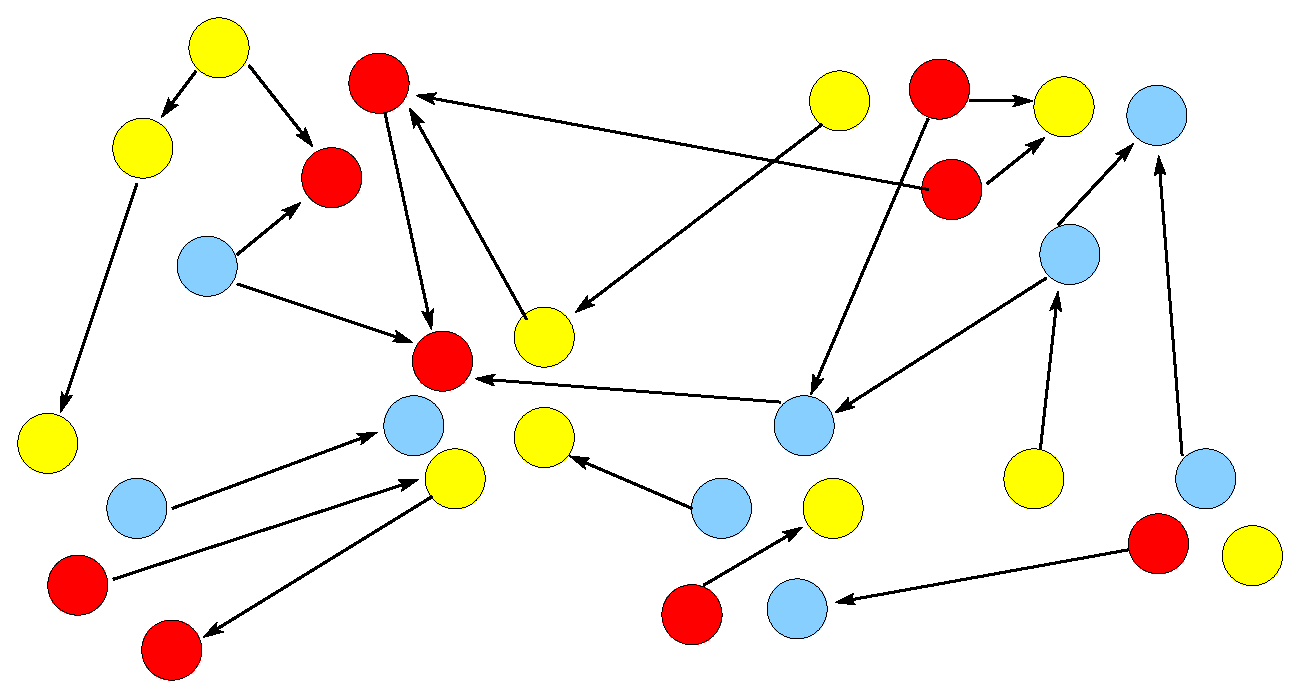
\includegraphics[width=0.7\linewidth]{gm.eps}
        \caption{แบบจำลองเชิงกราฟ}
    \end{center}
\end{figure}

\begin{figure}[h!]
    \begin{center}
        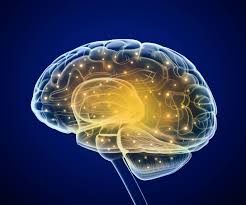
\includegraphics[width=0.5\linewidth]{brain.jpg}
        \caption{สภาพการเชื่อมโยงของสมอง (ที่มา: Shutterstock.com รูปโดย: Alex Mit)}
    \end{center}
\end{figure}

\begin{figure}
    \centering
    \subfigure[first caption]{ 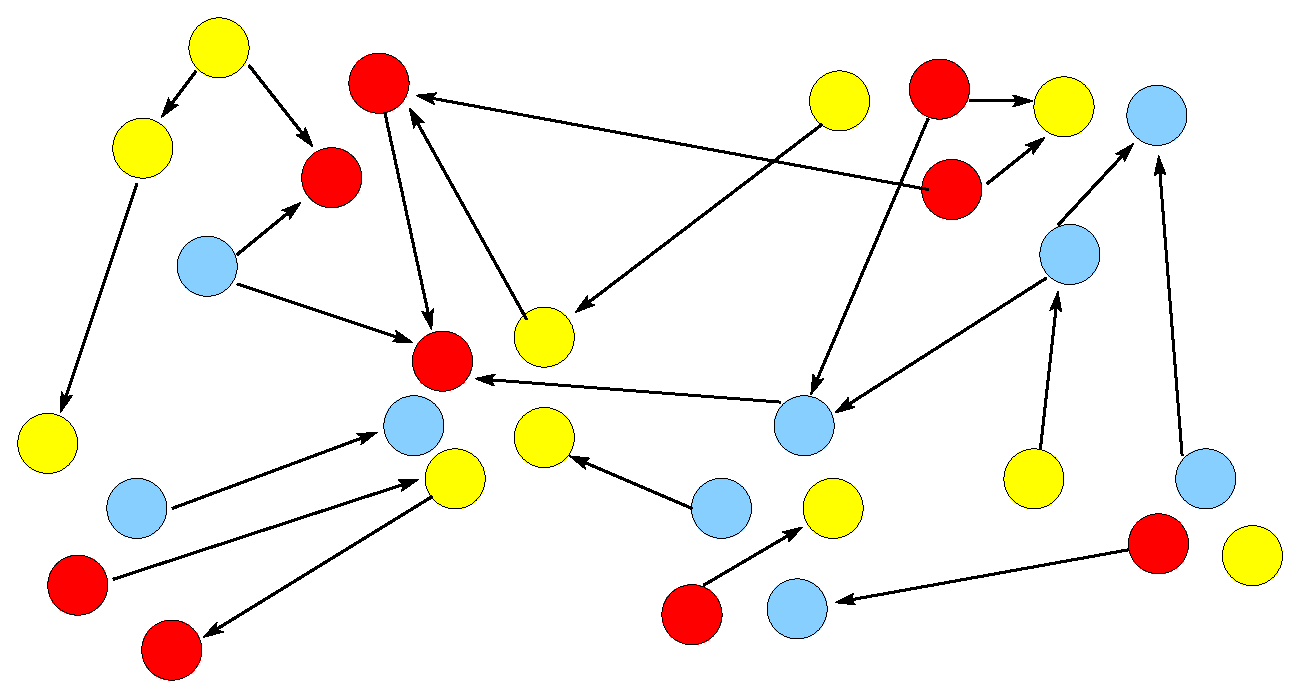
\includegraphics[width=0.45\linewidth]{gm.eps}  }
    \subfigure[second caption]{ 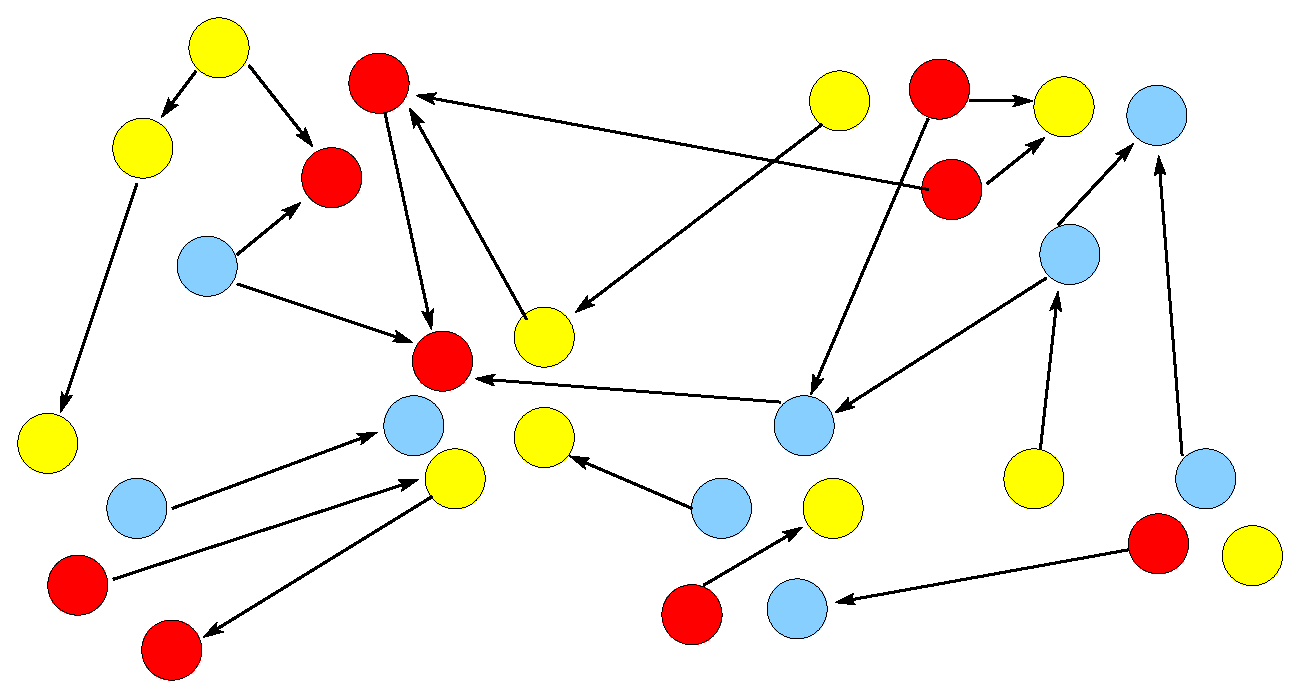
\includegraphics[width=0.45\linewidth]{gm.eps}  }
    \caption{ตัวอย่างการใช้ subfigure}
\end{figure}

\subsection{การพิมพ์สมการ}
กรณีพิมพ์สมการมีทั้งที่แทรกในบรรทัด เช่น $y=Cx$ หรือการแยกเป็นบรรทัดใหม่
\begin{equation}
    F(s) = \int_0^\infty e^{-st} f(t) dt
\end{equation}

การใช้ package 'align' จะสามารถเขียนสัญลักษณ์ต่างๆ ได้มากกว่า 1 บรรทัด มีได้หลายคอลัมน์ และสามารถจัดเรียงตำแหน่งได้ด้วย เช่น
\begin{align}
    x & = 2 \label{eq:x}       \\
    y & = 3 \label{eq:y}       \\
    z & = x \times y \nonumber \\
      & = p \label{eq:results}
\end{align}
การไม่ใส่หมายเลขสมการ สามารถใช้คำสั่ง \texttt{\nonumber} หรือ \texttt{notag} ได้ โดยปกติแล้วหากไม่ใส่อะไรเลย สมการทุกสมการจะมีหมายเลขกำกับเสมอ หลักการใส่เลขสมการคือ จะใส่เลขสมการก็ต่อเมื่อสมการนั้นจะถูกอ้างถึงในภายหลัง ดังนั้นการอ้างอึง (cross reference) สามารถทำได้โดยใช้คำสั่ง \texttt{ref} หรือ \texttt{eqref} กับ \texttt{label} ตัวอย่างเช่น สมการ~\eqref{eq:x} กล่าวไว้ว่า $x=2$

package 'eqnarray' ก็จะเป็นอีก environment หนึ่งที่ใช้เรียงสมการออกเป็น array

\begin{eqnarray}
    \dot{x} &=& Ax + Bu \\
    y &=& Cx+Du
\end{eqnarray}

ถ้าหากมีสมการหลายบรรทัดและต้องการเรียงในแนว center ให้ใช้ package 'gather'
\begin{gather}
    y = \sum_{n=0}^100 0.5^n + \sin(2\pi n t) + \lim_{n \rightarrow \infty} \frac{\log n}{n} \\
    z = \lim_{t \rightarrow \infty} e^{-st} g(t)
\end{gather}

\subsection{การใส่เอกสารอ้างอิง}
รูปแบบการเขียนเอกสารอ้างอิง ให้อิงตามรูปแบบที่ใช้ในบทความวิชาการเดียวกันทั้งรายงาน การอ้างอิงถึงเอกสารต่างชนิดกัน (เช่น หนังสือ บทความที่ตีพิมพ์ในวารสารวิชาการ บทความที่นำเสนอในที่ประชุมวิชาการ วิทยานิพนธ์) จะมีรูปแบบการอ้างอิงที่ต่างกัน และเป็นไปตามความนิยมหรือมาตรฐานต่าง ๆ ตัวอย่างรูปแบบการอ้างอิงแบบหนึ่งที่เป็นที่นิยมใช้มากในสาขาวิศวกรรมไฟฟ้าคือ รูปแบบการอ้างอิงของ IEEE ตามเอกสาร

\url{https://ieee-dataport.org/sites/default/files/analysis/27/IEEE Citation Guidelines.pdf}

การเรียงลำดับรายการเอกสารอ้างอิงแบบ IEEE ให้เรียงตามการอ้างถึงในเนื้อหารายงาน (อ้างถึงก่อนใช้ตัวเลขน้อย อ้างถึงทีหลังใช้ตัวเลขที่มากกว่า) โดยรายการเอกสารอ้างอิงดังข้างต้น ต้องปรากฏอยู่ในเนื้อความภายในรายงานด้วย (ไม่ต้องใส่เอกสารอ้างอิงที่ไม่ได้มีการอ้างถึงในรายงาน)


เอกสารอ้างอิงจะทำได้โดยง่าย หากใช้ \texttt{bibtex} โดยหลักการคร่าวๆ คือต้องมีไฟล์ฐานข้อมูลของเอกสารอ้างอิง เก็บในรูปแบบ \texttt{file.bib} ซึ่งบรรจุรหัสของเอกสารอ้างอิงที่ผู้ใช้ตั้งเอง และรายละเอียดของเปเปอร์นั้นๆ (สร้างได้โดยง่ายจากการใช้ Google Scholar ช่วย) ตัวอย่างการใช้งานคือ การใช้คำสั่ง \texttt{cite} เมื่อต้องการจะอ้างถึงเอกสารนั้นๆ เช่น หลักการ system identification เบื้องต้นนั้นสามารถอ่านได้จาก~\cite{SoS:89} เป็นต้น

\bibliography{ref}
\bibliographystyle{ieeetr}

\section{ภาคผนวก (ถ้ามี)}
ภาคผนวกเป็นข้อความที่ไม่สามารถใส่ไว้ในเนื้อหาหลักได้ แต่สามารถทำให้ผู้อ่านเข้าใจรายละเอียดของโครงงานได้มากยิ่งขึ้น ในหัวข้อนี้ให้ใส่รายละเอียดหรือข้อมูลอื่นๆ ที่จำเป็น ซึ่งไม่สำคัญเท่ากับที่อยู่ในเนื้อหาหลัก เช่น

\begin{itemize}
    \item ทฤษฎีพื้นฐานเพิ่มเติม เพื่อให้ผู้อ่านเข้าใจวิธีการที่ใช้ในโครงงานได้ดีขึ้น แต่การไม่ใส่รายละเอียดนี้ต้องไม่ทำให้ผู้อ่านไม่สามารถติดตามหรือเข้าใจเนื้อหาหลักได้
    \item Data Sheet ของอุปกรณ์ที่เลือกใช้
    \item Specification ของฮาร์ดแวร์ต่างๆ
    \item Features ของซอฟต์แวร์ที่ใช้
    \item Source Code ของโปรแกรมที่ได้เขียนขึ้นมาเอง หรือดัดแปลงมา
    \item Device Characteristics ของชิ้นส่วนในโครงงาน
\end{itemize}

ภาคผนวกอาจแบ่งออกเป็นหลายส่วน ตามหัวข้อเรื่อง เช่น

\subsection{ภาคผนวก ก.}

\subsection{ภาคผนวก ข.}

\end{document}